\section{Resultados}
	Para comprobar la funcionalidad del programa, primero probaré ingresando un AFD y posteriormente un AFND
	\paragraph{AFD}
	El AFD que creará nuestra clase AFD es el siguiente:
	\begin{figure}[H]
		\begin{center}
			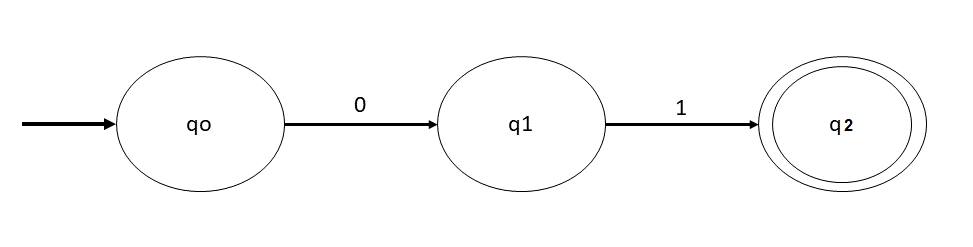
\includegraphics[width=10cm, height=4cm]{img/afd_auto.png}
			\caption{AFD de Prueba}
			\label{fig:tablas}
		\end{center}
	\end{figure}
	Este autómata solo acepta la cadena '01'. Cualquier otra cadena sería invalida.\\
	El archivo de entrada para la creación de este autómata, luce de la siguiente manera:
	\begin{figure}[H]
		\begin{center}
			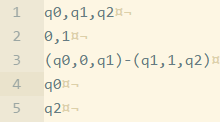
\includegraphics[width=6cm, height=4cm]{img/afd_entrada.png}
			\caption{Archivo de entrada para el AFD}
			\label{fig:tablas}
		\end{center}
	\end{figure}
	Al ejecutar el programa e ingresar el archivo, y posteriormente las cadenas, obtenemos las salidas esperadas.
	\begin{figure}[H]
		\begin{center}
			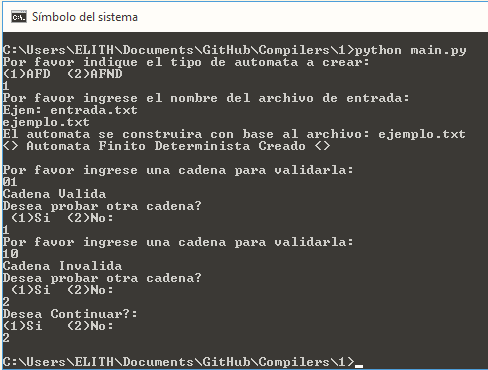
\includegraphics[width=15cm, height=10cm]{img/afd_salida.png}
			\caption{Ejecución y pruebas del AFD}
			\label{fig:tablas}
		\end{center}
	\end{figure}
	\newpage
	\paragraph{AFND}
	El AFND que creará nuestra clase AFND es el siguiente:
	\begin{figure}[H]
		\begin{center}
			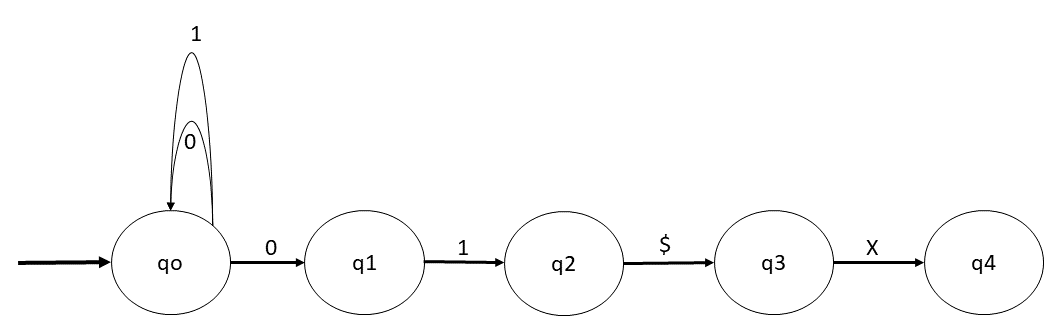
\includegraphics[width=10cm, height=4cm]{img/afnd_auto.png}
			\caption{AFND de Prueba}
			\label{fig:tablas}
		\end{center}
	\end{figure}
	Cabe señalar, que las transiciones epsilon son representadas por el símbolo '\textdollar'.\\
	Este autómata acepta la cadena '001x' por ejemplo, en general acepta cualquier cadena la cual empiece con cualquier cantidad de '0' o '1' pero que siempre al final lleve la siguiente combinación '1x'. Cualquier otra cadena sería invalida, por ejemplo, cadena '00x1'.\\
	El archivo de entrada para la creación de este autómata, luce de la siguiente manera:
	\begin{figure}[H]
		\begin{center}
			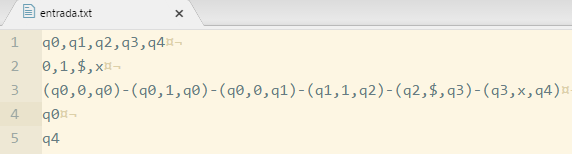
\includegraphics[width=12cm, height=5cm]{img/afnd_entrada.png}
			\caption{Archivo de entrada para el AFND}
			\label{fig:tablas}
		\end{center}
	\end{figure}
	\newpage
	Al ejecutar el programa e ingresar el archivo, y posteriormente las cadenas, obtenemos las salidas esperadas.
	\begin{figure}[H]
		\begin{center}
			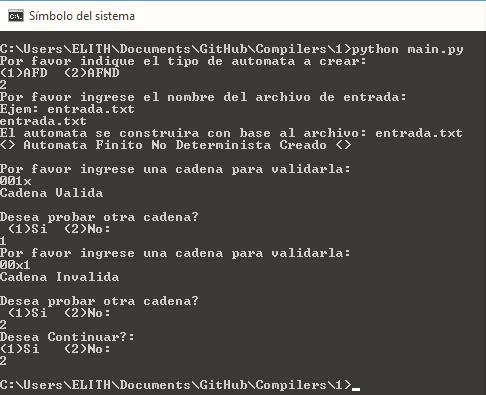
\includegraphics[width=15cm, height=10cm]{img/afnd_salida.png}
			\caption{Ejecución y pruebas del AFND}
			\label{fig:tablas}
		\end{center}
	\end{figure}